\section{Results and Discussion}

In this section, we report on the findings of our user study. Overall, we observed an increase in user engagement when comparing the proposed MindMargin interface against the traditional vertical commenting system. We were able to accept two of the three initially defined hypotheses.

Our first hypothesis predicted an overall increase in newly generated user comments, replies, upvotes, and downvotes when using MindMargin. We believed that having the comment system permanently visible on the side while reading an article, as in MindMargin, should increase these actions. However, this was not the case: we \textbf{rejected Hypothesis 1} since we did not observe an increase in the reading rate of comments or in interactions with comments when using our system. In fact, the participant group using MindMargin stated a 73\% reading rate of comments while the control group using the traditional interface stated a 85\% reading rate. In addition, there was no statistically significant increase in commenting rate, reply rate or the rate of up- and down-voting. We have several theories to explain these phenomena. First, we think that the users were overwhelmed by the number of existing comments. We populated both interfaces with 39 comments and replies, extracted from the original article. These comments covered a wide range of controversy regarding the content and participants might have thought that everything was already said. Second, since we were testing a rather unusual interface, we think that the novelty effect of introducing a new horizontal interface should not be underestimated. Third, because the study was hosted on an external site from that of the original article, which typically does not display news, participants may have concentrated more on reading the article than providing comments. Fourth, we do not know the number of comments that participants who reported to have read the comments did actually read.

Our second hypothesis was defined as an increase in personal reflection when using MindMargin. Exposure to a range of controversial comments should result in the rethinking and revising of one’s own opinions. All participants were asked their stance, from Strongly For TFA to Strongly Against TFA, on a Likert scale. Using data from participants who reported to have read the comments (see above), we observed the percentage of participants who claimed a strong stance on the article. Of those assigned to the MindMargin interface, only 16\% reported to be either Strongly For TFA or Strongly Against TFA. In contrast, 26\% of the participants using the traditional commenting system reported either extreme stance. The distribution of the Likert values is also normal for MindMargin and a U-shaped curve for the traditional commenting system. We performed a Shapiro-Wilk normality test ($alpha=0.05$) on both distributions. MindMargin rejects the null-hypothesis with $p=0.1306$ and therefore is normally distributed. The traditional prototype accepts the null-hypothesis with $p=0.0205$ and is therefore not normally distributed. We created Normal Q-Q plots for both (figures \ref{fig:mm_normal} and \ref{fig:reg_normal}). This reveals that despite no increase in the rate of reading comments, the MindMargin interface was able to encourage users to consider other opinions and viewpoints. This suggests a greater user engagement with the comments with the MindMargin interface. Therefore, we have \textbf{accepted Hypothesis 2}.

\begin{figure}[h]
\centering
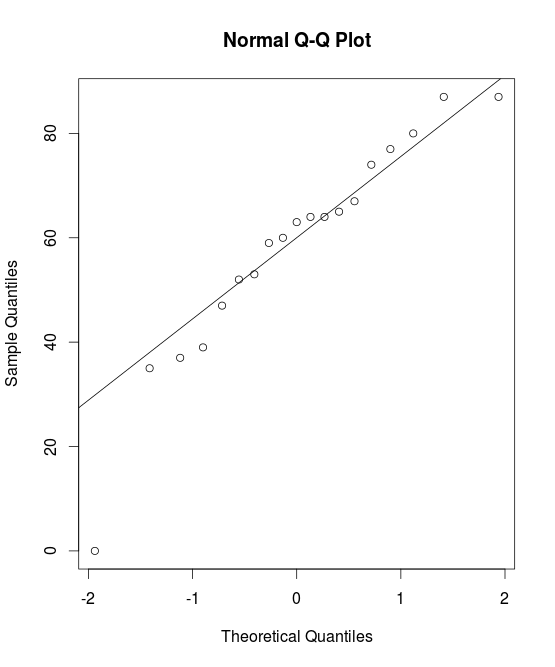
\includegraphics[scale=0.25]{mm_normal.png}
\caption{The personal stance distribution for MindMargin participants (normally distributed according to the Shapiro-Wilk normality test with $alpha=0.05$, $p=0.1306$).}
\label{fig:mm_normal}
\end{figure}

\begin{figure}[h]
\centering
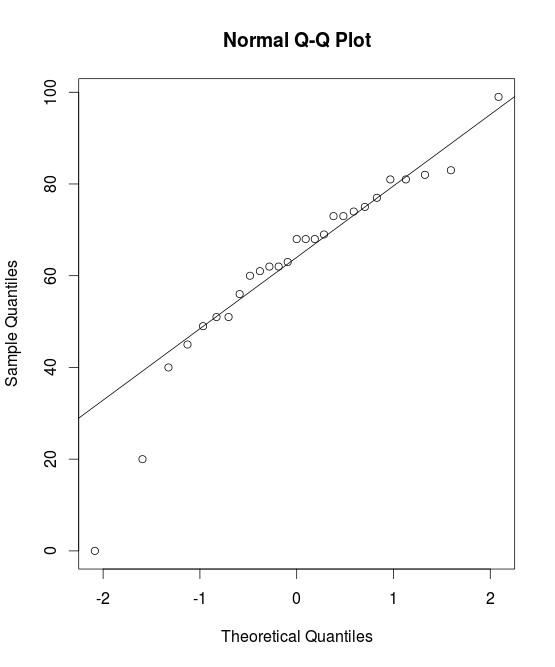
\includegraphics[scale=0.25]{regular_normal.png}
\caption{The personal stance distribution for traditional interface participants (normally distributed according to the Shapiro-Wilk normality test with $alpha=0.05$, $p=0.0205$).}
\label{fig:reg_normal}
\end{figure}

Our third hypothesis predicted an overall increase in positive impressions on comments when using the MindMargin interface. We asked participants who read the comments to input two adjectives in free-text describing either their reaction to the comments or a description of the comments. We then classified these adjectives using a three-bin classifier (“Positive,” “Negative,” and “Neutral”). “Positive” was assigned to positive reactions to comments, such as “interesting,” “well thought-out,” and “engaging.” “Negative” was assigned to negative reactions to comments, such as “annoying,” “useless,” “distracting.” “Neutral” was assigned to descriptive input about the comments, such as “long” and “subjective.” Finally, a few outliers, such as “trolls” and “whatever,” were removed. We observed a drastic change of impressions when using MindMargin. As seen in figure \ref{fig:trad_pie}, the majority of participants using the traditional commenting system described the comments as negative (68\%). In contrast, when using MindMargin, the majority of participants described the comments as positive (48\%) or neutral (48\%) as seen in figure \ref{fig:mm_pie}.  Outliers were also observed only to occur in the traditional commenting system. We have therefore \textbf{accepted Hypothesis~3}. 

\begin{figure}[h]
\centering
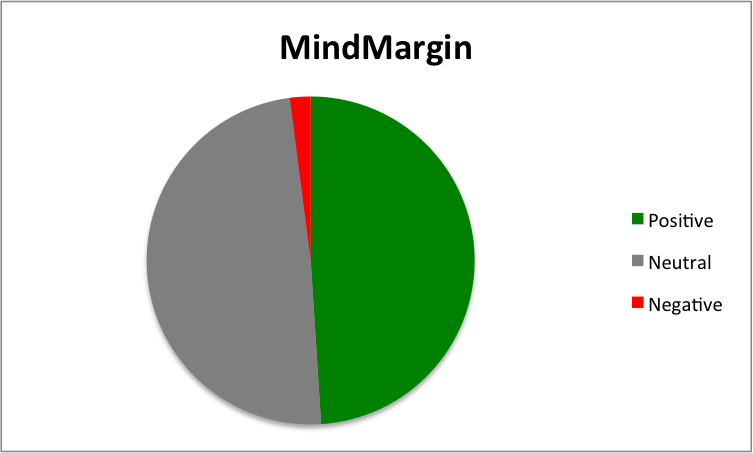
\includegraphics[scale=0.5]{mm_piechart.png}
\caption{When using MindMargin, the majority of participants described the comments as positive.}
\label{fig:mm_pie}
\end{figure}

\begin{figure}[h]
\centering
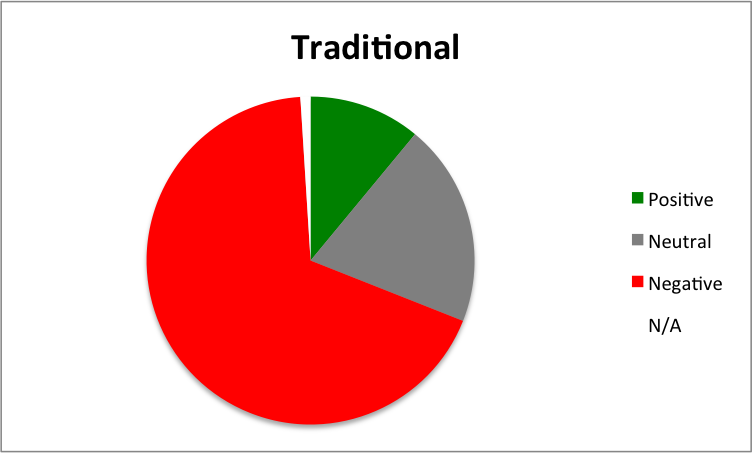
\includegraphics[scale=0.5]{traditional_piechart.png}
\caption{The majority of participants using the traditional commenting system described the comments as negative.}
\label{fig:trad_pie}
\end{figure}

The increased positive reaction to comments suggests that users perceive comments to be more substantial and worth greater consideration in the MindMargin interface. Even though participants were exposed to the identical comments and the comments were initially written for the traditional vertical interface, reactions to the comments were significantly more positive when using MindMargin. The rejection of Hypothesis 1 renders this finding even more surprising because there was no statistical difference in the number of people who read comments in either interface. The rejection ultimately supports the increase in user engagement with the MindMargin interface, and even suggests that MindMargin is not a distracting interface since participants can still opt out of reading comments if they so choose. Moreover, those who did not opt out of reading the comments found the exposure to anchored, relevant comments in MindMargin to be considerably more engaging and less distracting. In addition our quantitative results, we would like to quote qualitative feedback from a MindMargin user, suggesting actions he/she took beyond the scope of reading and commenting article: “This article showed me a new perspective on TFA, which after doing research, I have realized I agree with.” No feedback suggesting actions outside the scope of the article was received from participants with the traditional commenting system. 